\chapter{Конструкторская часть}

\section{Введение}
В данном разделе представлены схемы алгоритмов умножения матриц: стандартного, алгоритма Винограда и его оптимизированной версии, а также их теоретическая оценка трудоемкости.

\section{Разработка алгоритмов}
В данном разделе представлены схемы алгоритмов для стандартного умножения матриц (рисунок \ref{img:standart}), алгоритма Винограда умножения матриц (рисунки \ref{img:vinograd_alg_1} и \ref{img:vinograd_alg_2}) и оптимизированного алгоритма Винограда (рисунки \ref{img:vinograd_opt_alg_1} и \ref{img:vinograd_opt_alg_2}).

\begin{figure}[h]
	\centering
	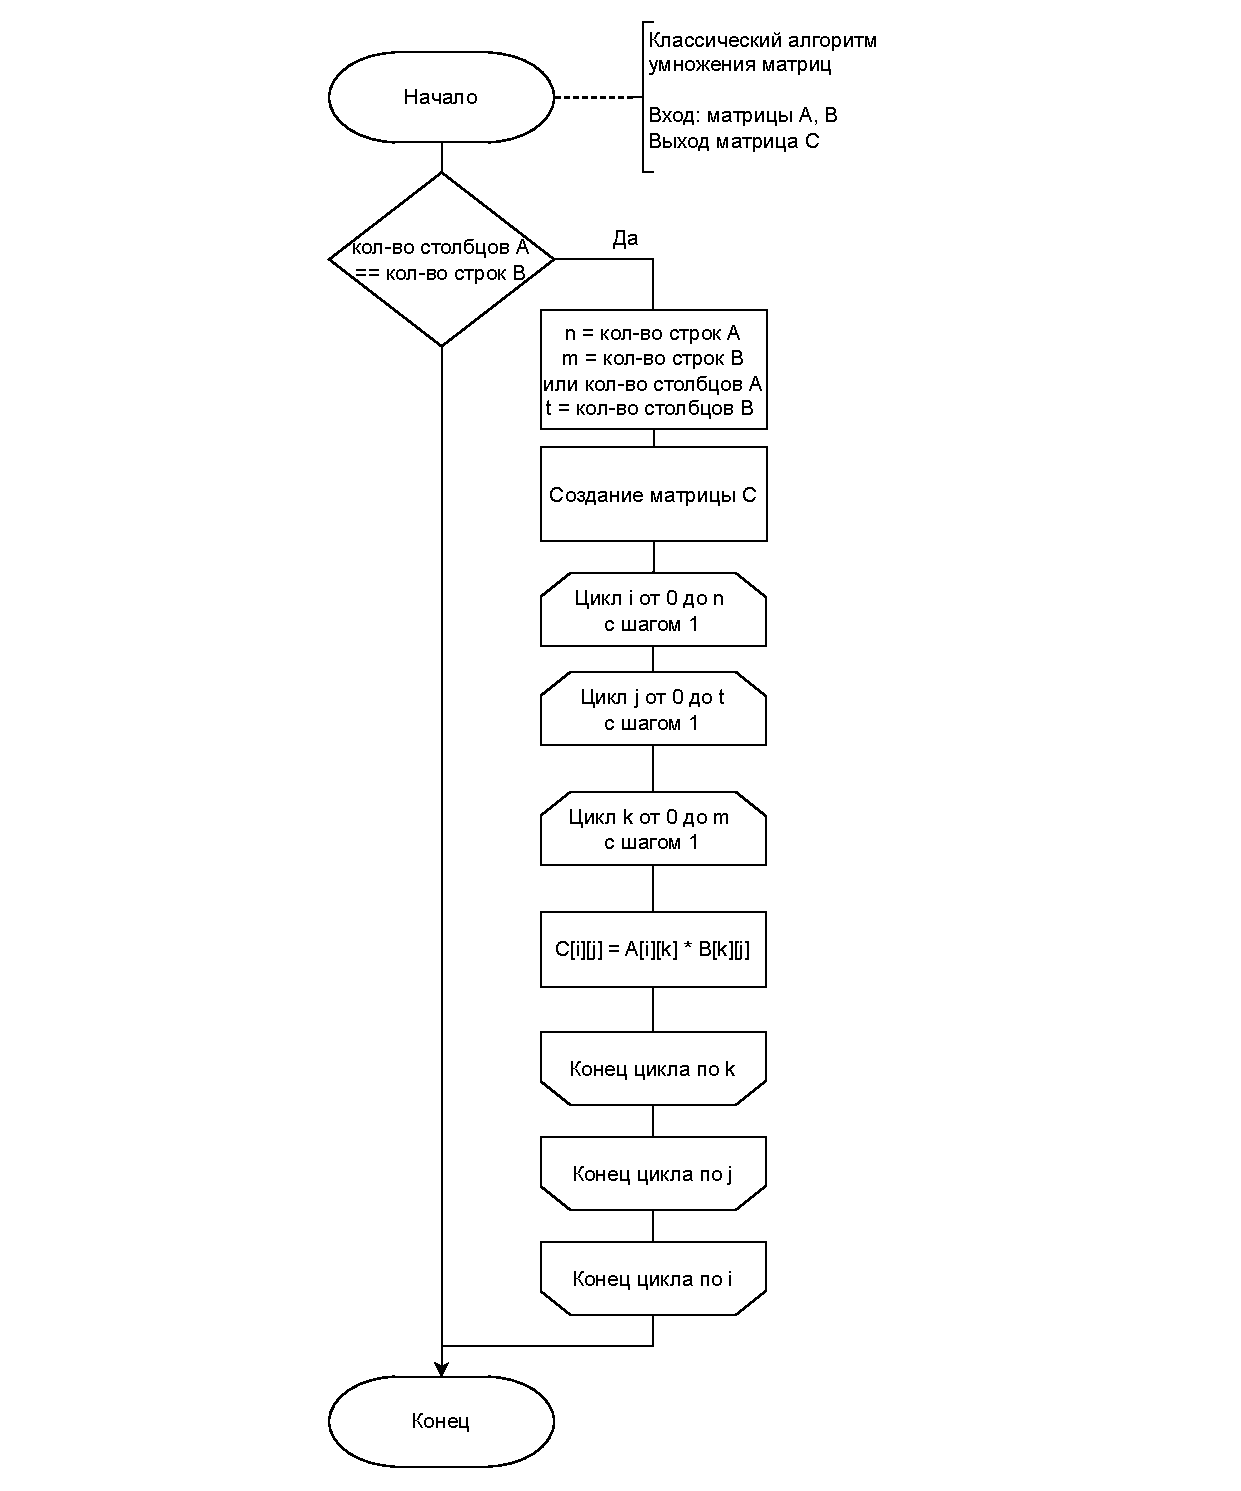
\includegraphics[width=1\linewidth]{img/standart.pdf}
	\caption{Схема стандартного алгоритма умножения матриц}
	\label{img:standart}
\end{figure}

\begin{figure}[h]
	\centering
	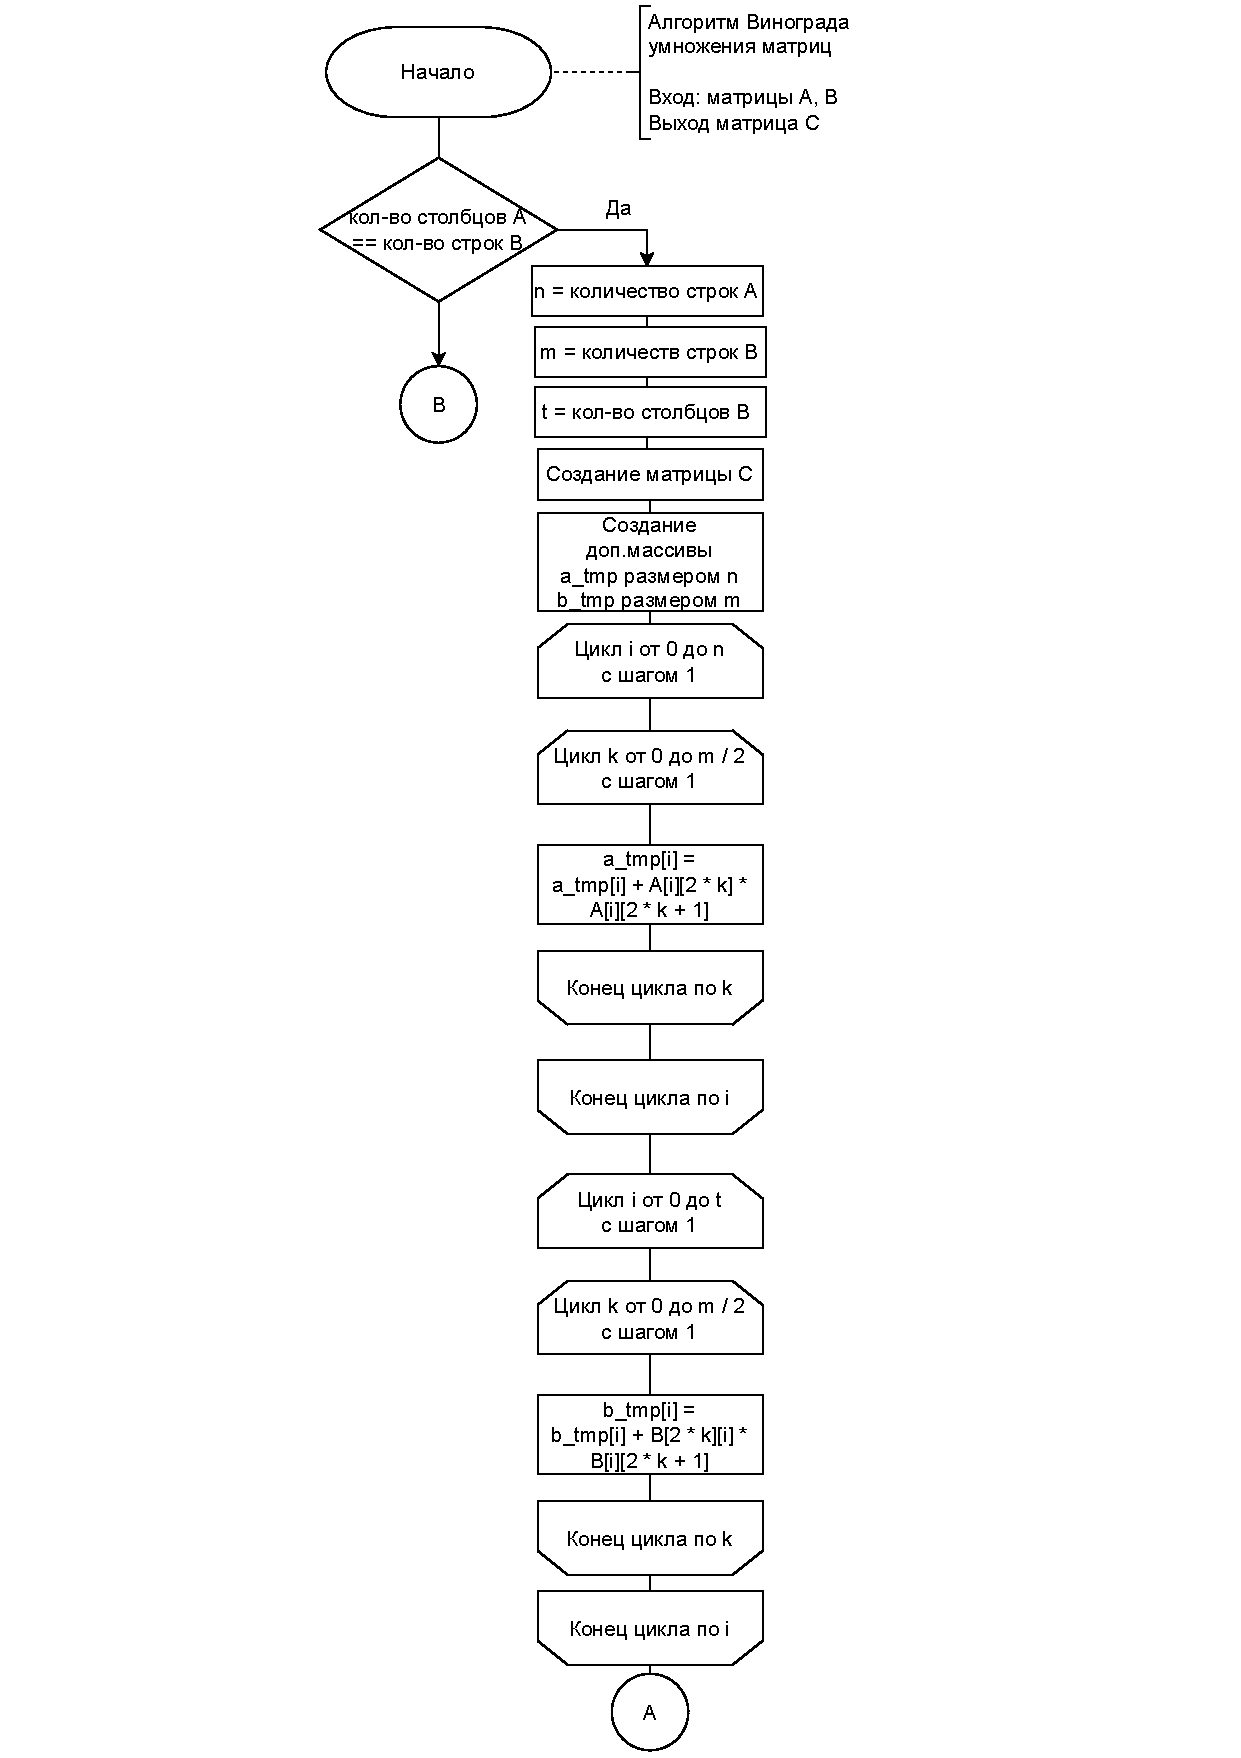
\includegraphics[width=1\linewidth]{img/vinograd_alg_1.pdf}
	\caption{Схема умножения матриц по алгоритму Винограда (Часть 1)}
	\label{img:vinograd_alg_1}
\end{figure}

\begin{figure}[h]
	\centering
	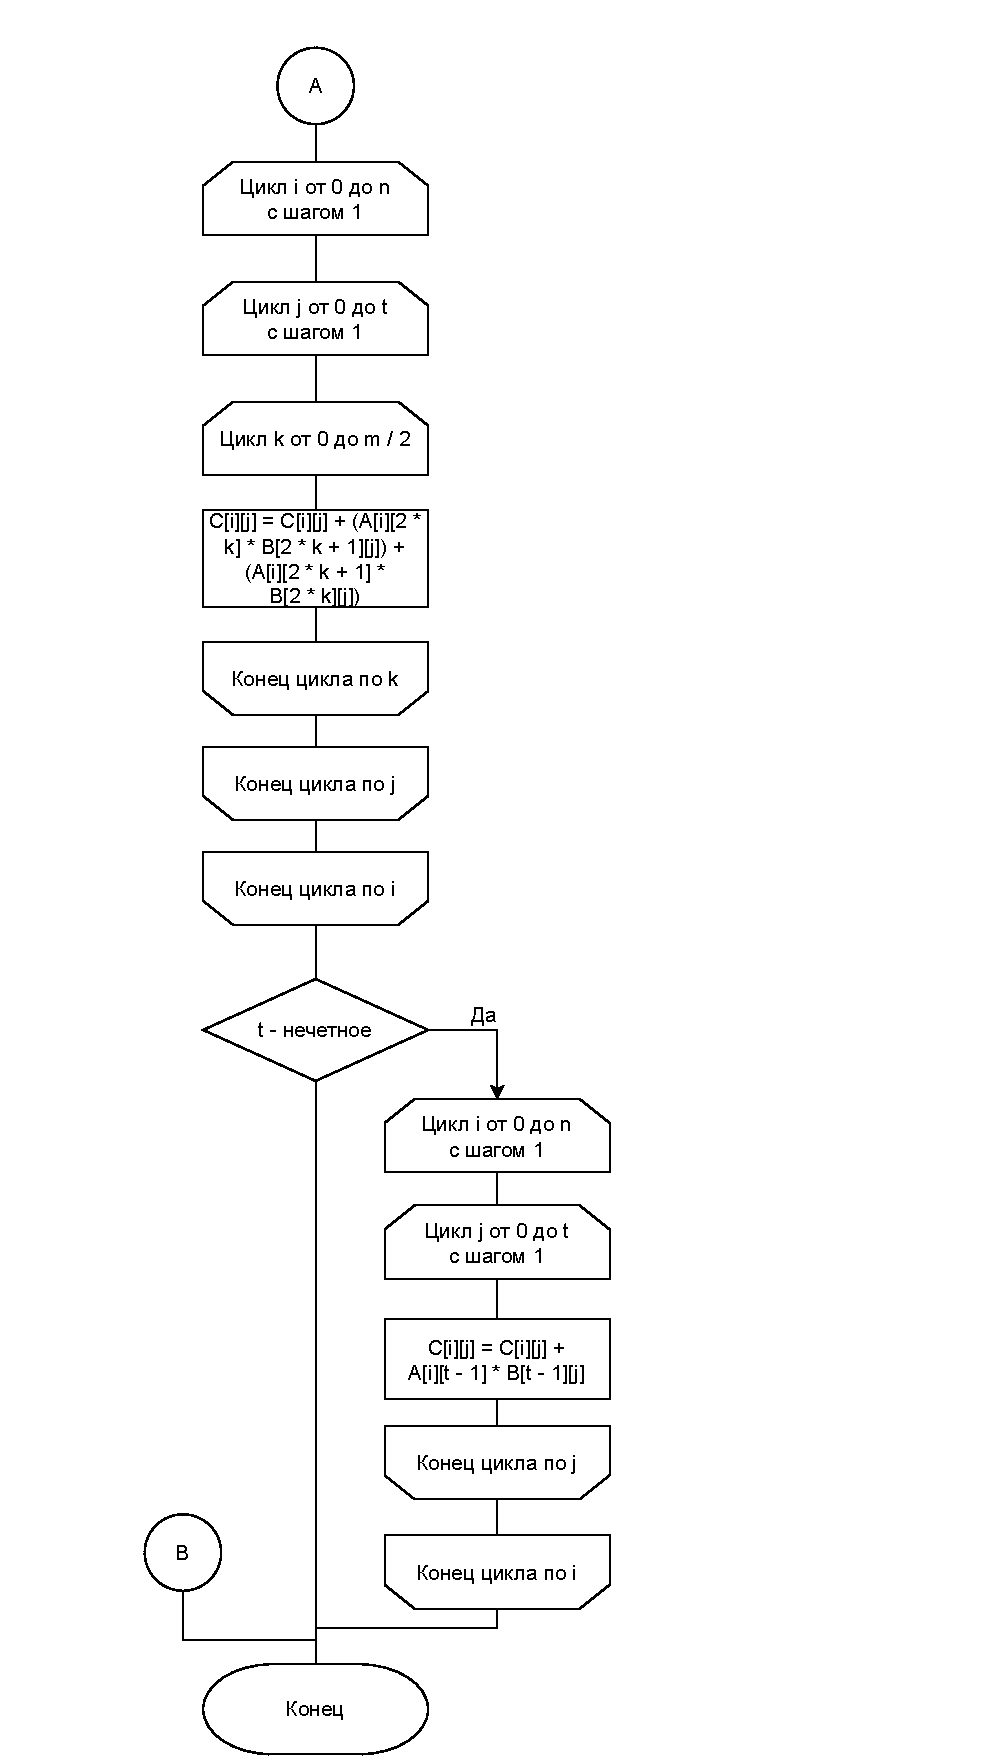
\includegraphics[width=0.8\linewidth]{img/vinograd_alg_2.pdf}
	\caption{Схема умножения матриц по алгоритму Винограда (Часть 2)}
	\label{img:vinograd_alg_2}
\end{figure}

\begin{figure}[h]
	\centering
	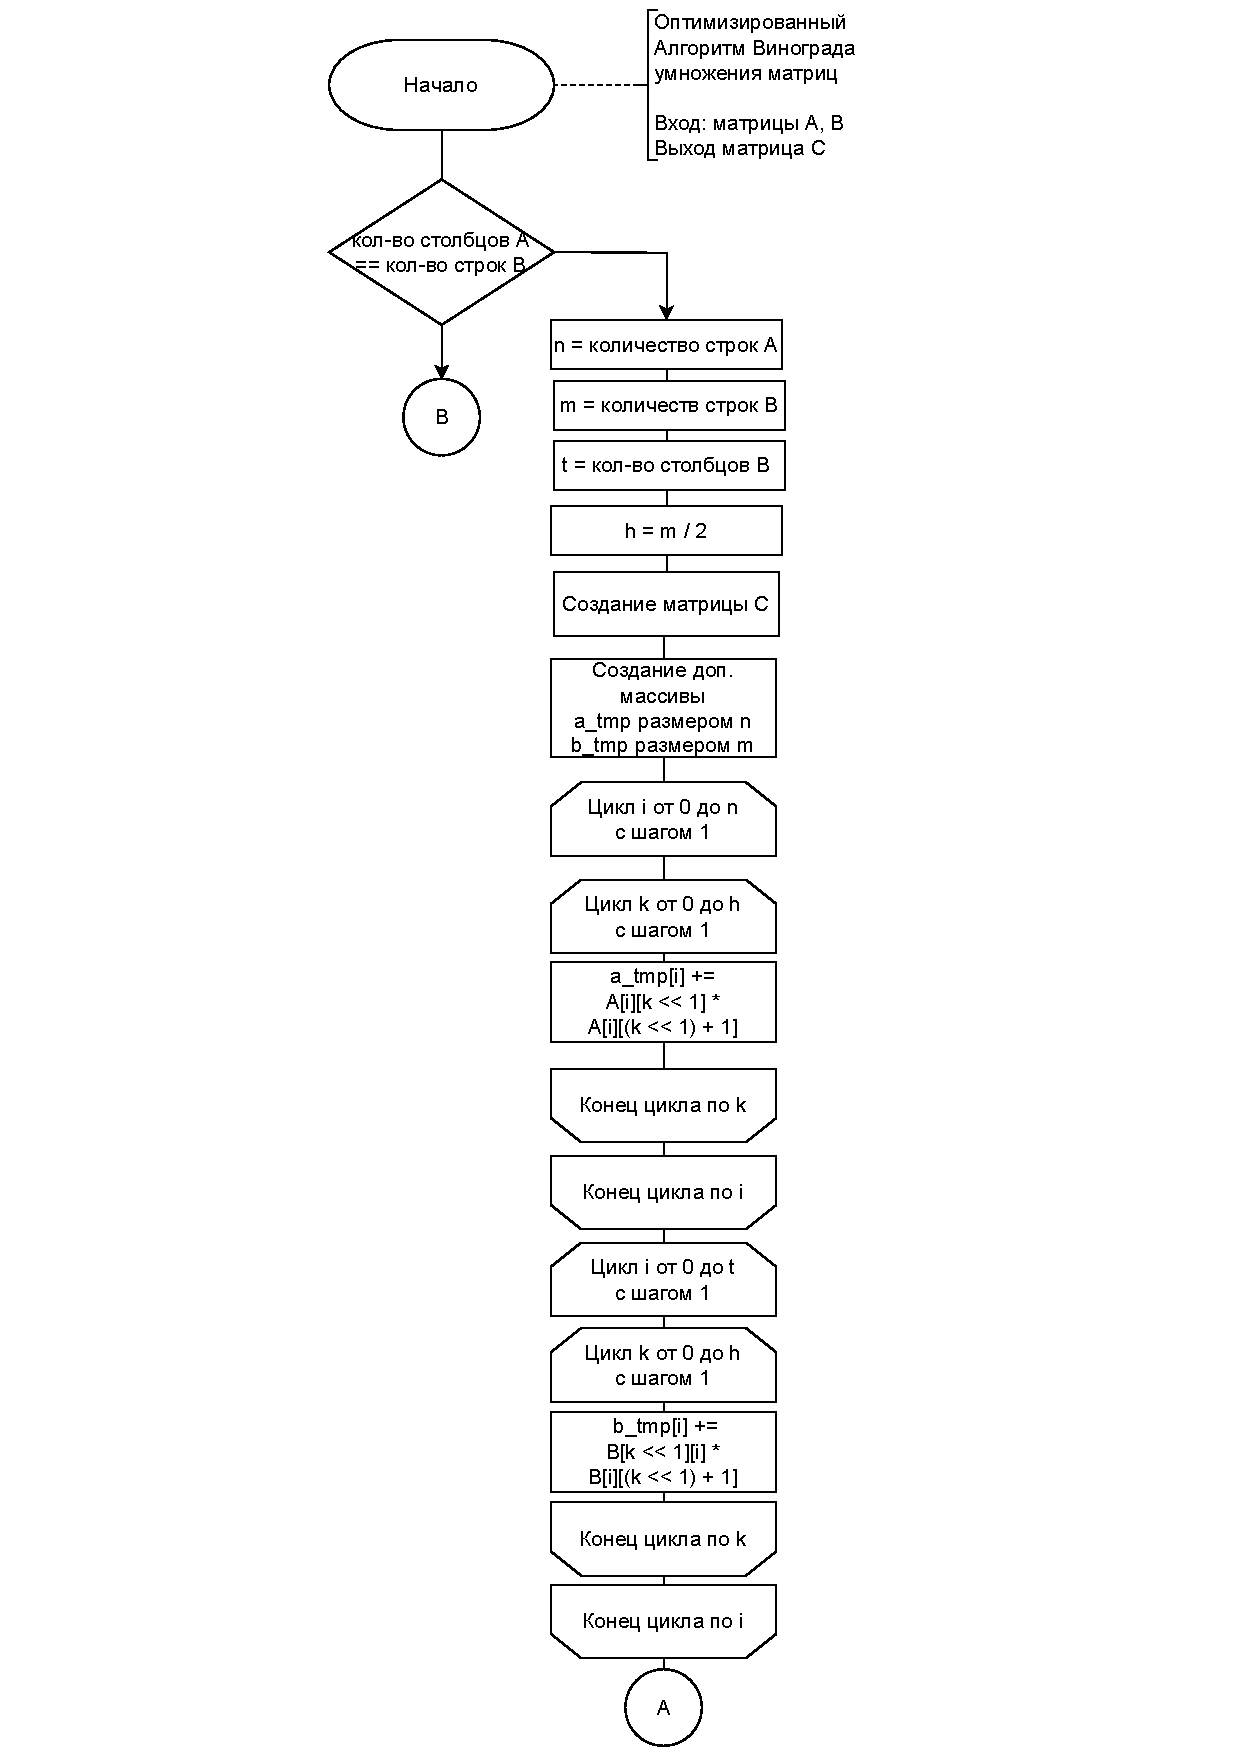
\includegraphics[width=1\linewidth]{img/vinograd_opt_alg_1.pdf}
	\caption{Схема умножения матриц по оптимизированному алгоритму Винограда (Часть 1)}
	\label{img:vinograd_opt_alg_1}
\end{figure}

\begin{figure}[h]
	\centering
	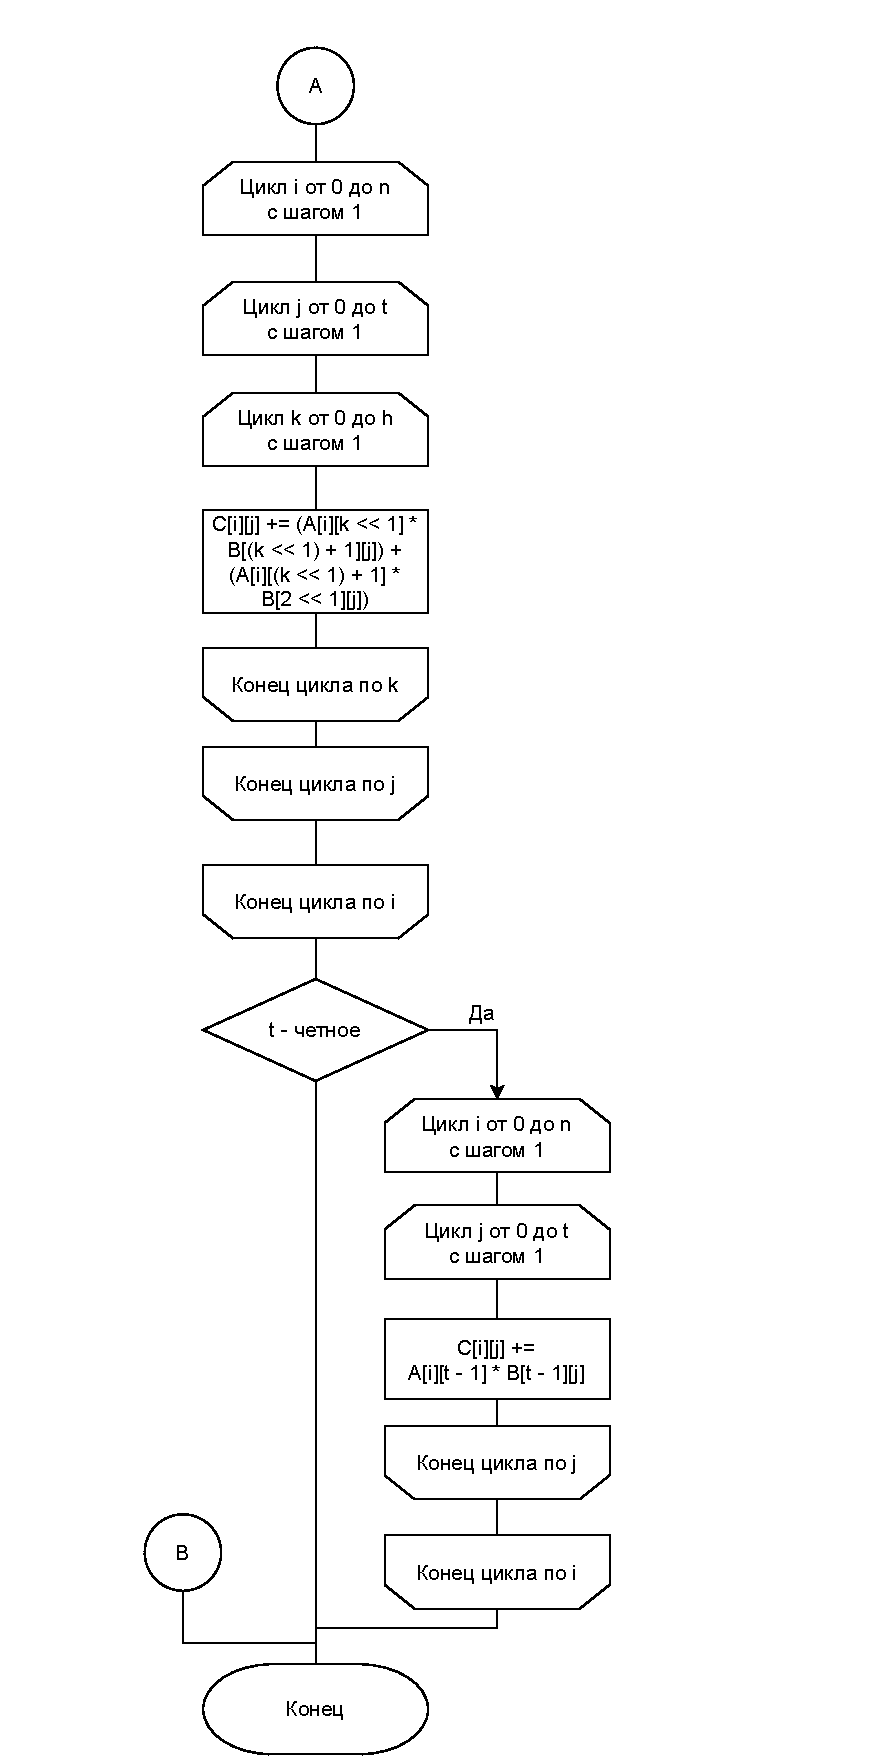
\includegraphics[width=0.7\linewidth]{img/vinograd_opt_alg_2.pdf}
	\caption{Схема умножения матриц по оптимизированному алгоритму Винограда (Часть 2)}
	\label{img:vinograd_opt_alg_2}
\end{figure}
\clearpage

\section{Модель вычислений для проведения оценки трудоемкости}

Введем модель вычислений, которая потребуется для определения трудоемкости каждого отдельного взятого алгоритма умножения матриц.
\begin{enumerate}[label={\arabic*)}]
	\item Трудоемкость базовых операций имеет:
	\begin{itemize}[label=---]
		\item равную 1:
		\begin{equation}
			\label{for:operations_1}
			\begin{gathered}
				+, -, =, +=, -=, ==, !=, <, >, <=, >=, [], ++, {-}-,\\
				\&\&, >>, <<, ||, \&, |
			\end{gathered}
		\end{equation}
		\item равную 2:
		\begin{equation}
			\label{for:operations_2}
			*, /, \%, *=, /=, \%=
		\end{equation}
	\end{itemize}
	\item Трудоемкость условного оператора:
	\begin{equation}
		\label{for:if}
		f_{if} = f_{\text{условия}} + 
		\begin{cases}
			min(f_1, f_2), & \text{лучший случай}\\
			max(f_1, f_2), & \text{худший случай}
		\end{cases}
	\end{equation}
	\item Трудоемкость цикла:
	\begin{equation}
		\label{for:for}
		\begin{gathered}
			f_{for} = f_{\text{инициализация}} + f_{\text{сравнения}} + M_{\text{итераций}} \cdot (f_{\text{тело}} +\\
			+ f_{\text{инкремент}} + f_{\text{сравнения}})
		\end{gathered}
	\end{equation}
	\item Трудоемкость передачи параметра в функции и возврат из функции равны 0.
\end{enumerate}

\section{Трудоемкость алгоритмов}

Была рассчитана трудоемкость алгоритмов умножения матриц.

\subsection{Классический алгоритм}

Для стандартного алгоритма умножения матриц трудоемкость будет слагаться из:

\begin{itemize}[label=---]
	\item внешнего цикла по $i \in [1 \ldots N]$ , трудоёмкость которого: $f = 2 + N \cdot (2 + f_{body})$;
	\item цикла по $j \in [1 \ldots T]$ , трудоёмкость которого: $f = 2 + 2 + T \cdot (2 + f_{body})$;
	\item цикла по $k \in [1 \ldots M]$ , трудоёмкость которого: $f = 2 + 2 + 14M$;
\end{itemize}

Поскольку трудоемкость стандартного алгоритма равна трудоемкости внешнего цикла, то:
\begin{equation}
	\label{сomplexity:standart}
	\begin{gathered}
		f_{standart} = 2 + N \cdot (2 + 2 + T \cdot (2 + 2 + M \cdot (2 + 8 + 1 + 1 + 2)))= \\
		= 2 + 4N + 4NT + 14NMT \approx 14NMT = O(N^3)
	\end{gathered}
\end{equation}

\clearpage

\subsection{Алгоритм Винограда}

Чтобы вычислить трудоемкость алгоритма Винограда, нужно учесть следующее:
\begin{itemize}[label=---]
	\item создания и инициализации массивов $a_{tmp}$ и $b_{tmp}$, трудоёмкость которых указана в формуле~(\ref{сomplexity:v_init});
	\begin{equation}
		\label{сomplexity:v_init}
		f_{init} = N + M
	\end{equation}
	\item заполнения массива $a_{tmp}$, трудоёмкость которого указана в формуле~(\ref{сomplexity:v_atmp});
	\begin{equation}
		\label{сomplexity:v_atmp}
		\begin{gathered}
			f_{atmp} = 2 + N \cdot (4 + \frac{M}{2} \cdot (4 + 6 + 1 + 2 + 3 \cdot 2)) = \\
			= 2 + 4N + \frac{19NM}{2} = 2 + 4N + 9,5NM
		\end{gathered} 
	\end{equation}
	\item заполнения массива $b_{tmp}$, трудоёмкость которого указана в формуле~(\ref{сomplexity:v_btmp});
	\begin{equation}
		\label{сomplexity:v_btmp}
		\begin{gathered}
			f_{btmp} = 2 + T \cdot (4 + \frac{M}{2} \cdot (4 + 6 + 1 + 2 + 3 \cdot 2)) = \\
			= 2 + 4T + \frac{19TM}{2} = 2 + 4T + 9,5TM
		\end{gathered}  
	\end{equation}
	\item цикла заполнения для чётных размеров, трудоёмкость которого указана в формуле~(\ref{сomplexity:v_cycle});
	\begin{equation}
		\label{сomplexity:v_cycle}
		\begin{gathered}
			f_{cycle} = 2 + N \cdot (4 + T \cdot (2 + 7 + 4 + \frac{M}{2} \cdot (4 + 28))) = \\
			= 2 + 4N + 13NT + \frac{32NTM}{2}  = 2 + 4N + 13NT + 16NTM 
		\end{gathered}
	\end{equation}
	\item цикла, который дополнительно нужен для подсчёта значений при нечётном размере матрицы, трудоемкость которого указана в формуле~(\ref{сomplexity:v_check});
	\begin{equation}
		\label{сomplexity:v_check}
		\begin{gathered}
			f_{check} = 3 + 
			\begin{cases}
				0, & \text{чётная} \\
				2 + N \cdot (4 + T \cdot (2 + 14)), & \text{иначе}
			\end{cases}
		\end{gathered}  
	\end{equation}
\end{itemize}

Тогда для худшего случая (нечётный общий размер матриц) имеем:
\begin{equation}
	\label{сomplexity:vinograd_worst}
	\begin{gathered}
		f_{worst} = f_{init} + f_{atmp} + f_{btmp} + f_{cycle} + f_{check} \approx 16NMT = O(N^3)
	\end{gathered}
\end{equation}

Для лучшего случая (чётный общий размер матриц) имеем:
\begin{equation}
	\label{сomplexity:vinograd_best}
	\begin{gathered}
		f_{best} = f_{init} + f_{atmp} + f_{btmp} + f_{cycle} + f_{check} \approx 16NMT = O(N^3)
	\end{gathered}
\end{equation}

\subsection{Оптимизированный алгоритм Винограда}

Трудоемкость оптимизированного алгоритма Винограда состоит из:
\begin{itemize}[label=---]
	\item кэширования значения $\frac{M}{2}$ в циклах, которое равно 3;
	\item создания и инициализации массивов $a_{tmp}$ и $b_{tmp}$ (\ref{сomplexity:v_init});
	\item заполнения массива $a_{tmp}$, трудоёмкость которого (\ref{сomplexity:v_atmp});
	\item заполнения массива $b_{tmp}$, трудоёмкость которого (\ref{сomplexity:v_btmp});
	\item цикла заполнения для чётных размеров, трудоёмкость которого указана в формуле (\ref{сomplexity:v_opt_cycle});
	\begin{equation}
		\label{сomplexity:v_opt_cycle}
		\begin{aligned}
			f_{cycle} = 2 + N \cdot (4 + T \cdot (4 + 7 + \frac{M}{2} \cdot (2 + 10 + 5 + 2 + 4))) = \\
			= 2 + 4N + 11NT + \frac{23NTM}{2}  =\\
			= 2 + 4N + 11NT + 11,5 \cdot NTM 
		\end{aligned}
	\end{equation}
	\item условие, которое нужно для дополнительных вычислений при нечётном размере матрицы, трудоемкость которого указана в формуле~(\ref{сomplexity:v_opt_check});
	\begin{equation}
		\label{сomplexity:v_opt_check}
		\begin{aligned}
			f_{check} = 3 + 
			\begin{cases}
				0, & \text{чётная} \\
				2 + N \cdot (4 + T \cdot (2 + 10)), & \text{иначе}
			\end{cases}
		\end{aligned}  
	\end{equation}
\end{itemize}

Тогда для худшего случая (нечётный общий размер матриц) имеем:
\begin{equation}
	\label{сomplexity:vinograd_opt_worst}
	\begin{aligned}
		f_{worst} = 3 + f_{init} + f_{atmp} + f_{btmp} + f_{cycle} + f_{check} \approx 11NMT = O(N^3)
	\end{aligned}
\end{equation}

Для лучшего случая (чётный общий размер матриц) имеем:
\begin{equation}
	\label{сomplexity:vinograd_opt_best}
	\begin{aligned}
		f_{best} = 3 + f_{init} + f_{atmp} + f_{btmp} + f_{cycle} + f_{check} \approx 11NMT = O(N^3)
	\end{aligned}
\end{equation}

\section*{Вывод}
В данном разделе были представлены схемы алгоритмов умножения матриц и проведена теоретическая оценка трудоемкости алгоритмов. 
Результаты показывают, что оптимизированный алгоритм Винограда позволяет добиться уменьшения трудоемкости в 1.2 раза.